\documentclass[12pt]{cutecv}
\usepackage[english]{babel}
\usepackage{hyperref}
\usepackage{graphicx}

\newcommand{\listbullet}{$\; \cdot \;$}

\author{Ksenia Syrbulova}
\contacts{tg: @naysudes | +79639699628 | syrbulova@gmail.com}
\begin{document}

\maketitle

\columnratio{0.3,0.7}
\begin{paracol}{2}
\setlength{\columnsep}{2em}
\setlength{\cvsectionverticalskip}{5mm}
\setlength{\cvinfoverticalskip}{5mm}

\begin{leftcolumn}
  \vspace{5mm}
  \begin{figure}[htp]
    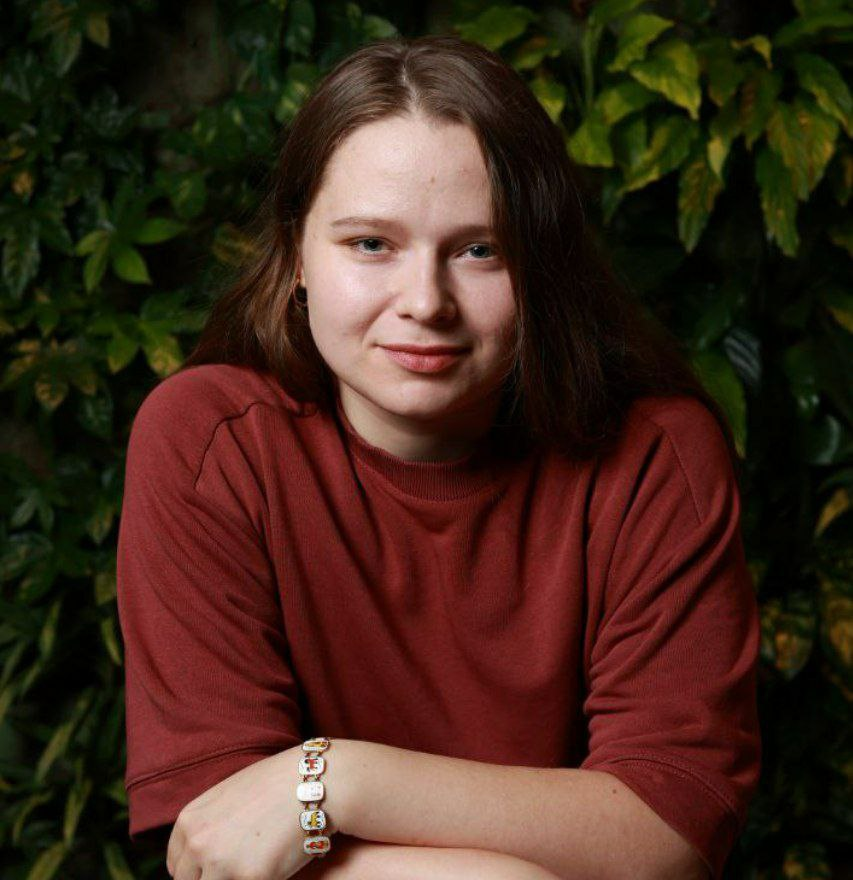
\includegraphics[width=5cm, height=5cm]{image.jpg}
\end{figure}

\begin{cvsection}{Key skills}
  \listbullet Backend \listbullet User-space networking \listbullet Algorithms \listbullet Databases
   \listbullet Distributed systems \listbullet Concurrency
   \listbullet Performance \\
\end{cvsection}

\begin{cvsection}{Languages}
  Golang \listbullet Python \listbullet C++
\end{cvsection}

\begin{cvsection}{Technologies}
  Linux \listbullet Kafka \listbullet RabbitMQ
  gRPC \listbullet PostgreSQL \listbullet  MongoDB \listbullet Docker \listbullet Kubernetes
  \listbullet Git \\
\end{cvsection}

\end{leftcolumn}

\begin{rightcolumn}
\begin{cvsection}{Experience (4 years)}
  \cvinfobox{Yandex.Taxi}{ 02.2022-present | Python Developer}
  {Developed Taxi Billing services. Supported new functionality (payment and netting pipelines), 
  optimized data processing and added auxiliary functionality (reconciliation of data uploads and payments). \\
  \underline{Technologies:} Python and C++ as programming languages, PostgreSQL and YDB as databases.\\
  \underline{Achievements:} \\ \listbullet Instant Payments for Drivers project, which
  were able to reduce the waiting time for payments to drivers' cards from 24 hours to 5 minutes.\\
  \listbullet Streaming reconciliations of data uploads, which prevented a financial incident of a large value.}
  
  \cvinfobox{Applied Logistics}{ 06.2020-02.2022 | С++ Developer}
  {Developed an accounting program for factory production facilities. We created a user-friendly interface, crash-proof and data-loss-proof system. \\
  \underline{Technologies:} C++, PostgreSQL. Qml and QT as frameworks for creating interfaces.\\
  \underline{Achievements:} independently developed the accounting module for one of the truck model and delivered it to customers without additional revisions.}
\end{cvsection}
\begin{cvsection}{Education}
  \cvinfobox{N.E. Bauman Moscow State Technical University}{2016-2020 | Applied mechanics}{Bachelor's degree in mechanical engineering}
  \cvinfobox{Technopark Mail.ru | VK Education}{2021-2022 | System architect}
    {Two years of full-stack engineer training, with courses in DB, frontend and backend, as well as SRE.}
  \cvinfobox{YANDEX SCHOOL OF DATA ANALYSIS}{2023-2024 | CS Track}{An in-depth course on Distributed Systems with diving into networking, database internals, and services exploitation.}
\end{cvsection}
\end{rightcolumn}
\end{paracol}

\end{document}
